\documentclass[]{article}
\usepackage[T1]{fontenc}
\usepackage{amsfonts}
\usepackage{graphicx}
\usepackage[linesnumbered,lined,boxed,commentsnumbered,ruled,vlined]{algorithm2e}

%opening
\title{Projekt Zespołowy \\
	\Huge Etap projektu – projektowanie rozwiązania na zadaną architekturę}
\author{\\ \\ \\ Autorzy:
	\\Biernacka Kamila\\ 
	Kania Dominik\\ 
	Leśniak Mateusz\\ 
	Maziarz Wojciech\\ \\ \\ \\ \\ \\ \\ \\ \\ \\ \\ \\ \\ \\ \\ \\ \\  }
\date{kwiecień 2021}

\begin{document}

\maketitle
\newpage

\begin{abstract}

Poniższe sprawozdanie jest wynikiem naszej pracy na drugim etapie projektu zespołowego z implementacji metody indeksu w architekturach GPU. Przedstawimy w nim przygotowane przez nas projekty i rysunki koncepcyjne wymaganych do zaimplementowania algorytmów.



\end{abstract}

\section{Analiza możliwości implementacji algorytmów mnożenia modularnego dużych liczb}
Zaproponowanym przez nas algorytmem jest ten odkryty przez rosyjskiego matematyka Anatolija Karacubę. Umożliwia on zmniejszenie złożoności czasowej ($\Theta(n^{log_{2}3})$) w porównaniu do mnożenia klasycznego ($\Theta(n^2)$) .
\newline\newline
~Projekt algorytmu:\newline

Mnożone są dwie \textit{n}-cyfrowe liczby \textit{x} i \textit{y} przy podstawie \textit{B}, gdzie \textit{n = 2m}. Przetwarzane \textit{n} może być nieparzyste, a \textit{x} i \textit{y} mogą mieć różną liczbę cyfr. W takim przypadku po lewej stronie tych liczb należy dopisać zera. Wartości \textit{x}~i~\textit{y}~należy rozpisać jako:\newline
$$ x = x_{1}B^{m} + x_2 $$
$$ y = y_{1}B^{m} + y_2, $$
gdzie $x_2$, $y_2$ < $B^m$. \newline
Przemnożenie tych liczb prowadzi do otrzymania równania:
$$xy = (x_{1}B^{m} + x_2)(y_1B^m + y_2) = x_1y_1B^{2m} + (x_1y_2 + x_2y_1)B^m + x_2y_2.$$ 
Klasycznie problem ten rozwiązuje się poprzez przemnożenie czterech czynników osobno, wykonanie przesunięcia i dodanie ich, co powoduje, że opisany algorytm wykonuje się w czasie $\textit{O}(n^{2})$. Karacuba zaproponował, by zastąpić go trzema mnożeniami:
$$X = x_1y_1$$
$$Y = x_2y_2$$
$$Z = (x_1 + x_2)(y_1 + y_2) - X - Y$$
W wyniku tego otrzymuje się równanie:
$$ Z = (x_1y_1 + x_1y_2 + x_2y_1 + x_2y_2) - x_1y_1 - x_2y_2 = x_1y_2 + x_2y_1.$$
Zatem $xy = XB^{2m} + Y + ZB^m$. Tak więc wystarczy zaledwie kilka dodatkowych dodawań i odejmowań, by zmniejszyć liczbę mnożeń z czterech do trzech.\newline
Algorytm można rozszerzyć i wykonać każde z tych mnożeń \textit{m}-cyfrowych liczb ponownie w ten sam sposób przy wykorzystaniu rekurencji.


\section{Analiza możliwości implementacji algorytmu poszukiwania relacji (oraz faktoryzacji w bazie), dla algorytmu metody indeksu}

\begin{algorithm}
	\SetAlgoLined
	\caption{Faktoryzacja, \(isFactored\)}
	\label{Faktor}
	\KwIn{\(x\), \(N\)}
	\KwOut{\(True\) lub \(False\)}
	\For{\(i \gets 0; \; i < len(N); \; i \gets i + 1\)}
	{
		\While{\(x \% N[i] == 0\)}
		{
			\(x \gets x/N[i]\)\\
		}
		\(i \gets i + 1\)
	}
	\If{\(x == 1\)}
	{
			\Return{\(True\)}
	}
	\Return{\(False\)}
\end{algorithm}

\begin{algorithm}
	\SetAlgoLined
	\caption{Poszukiwanie relacji}
	\label{Relation}
	\KwIn{\(\mathbb{B}\), \(l\)}
	\KwOut{\(N\), \(R\)}
	\(i \gets 0\) \\
	\While{\(p_i \leq \mathbb{B}\), \(p_i \in \mathcal{P}\)}
	{
		\(N[i] \gets p_i\)\\
		\(i \gets i + 1\)\\
	}
	\(j \gets 0\) \\
	\While{\(j < l\)}
	{
		\(x \gets random(\mathbb{F}_p^*)\)\\
		\If{\(isFactored(x, N)\)}
		{
			\(R[j] \gets x\)\\
			\(j \gets j + 1\)\\
		}
	}
	\Return{\(N, R\)}
\end{algorithm}


\section{Analiza możliwości implementacji algorytmu eliminacji Gaussa nad ciałem $\mathbb{F}_p$, dla ciał o dowolnym rozmiarze}~
	\begin{algorithm}
		\SetAlgoLined
		\caption{Poszukiwanie relacji}
		\label{Gauss}
		\KwIn{\(\mathbb{A}_{l,k}\)}
		\KwOut{\(x\)}
		\For{\(i \gets 0; \; i < l; \; i \gets i + 1\)}
		{
			\(w_{i,j} \gets \frac{\mathbb{A}_{j,i}}{\mathbb{A}_{i,i}}\)\\
			\For{\(j \gets 0; \; j < k-1; \; j \gets j + 1\)}
			{
				\(\)
			}
		}

	\end{algorithm}


\section{Metoda indeksu}~
	Metoda indeksu podzielona jest na 4 etapy. 
	\begin{enumerate}
		\item Konstruowanie zbioru relacji z wykorzystaniem algorytmu \ref{Relation}
		\item Rozwiązanie układu równań z wykorzystaniem algorytmu (ref do algorytmu eliminacji gaussa)
		\item Wyznaczenie wartości \(r\);
		\item Wyznaczenie rozwiązania;
	\end{enumerate}
	\begin{figure}[h]
		\begin{center}
			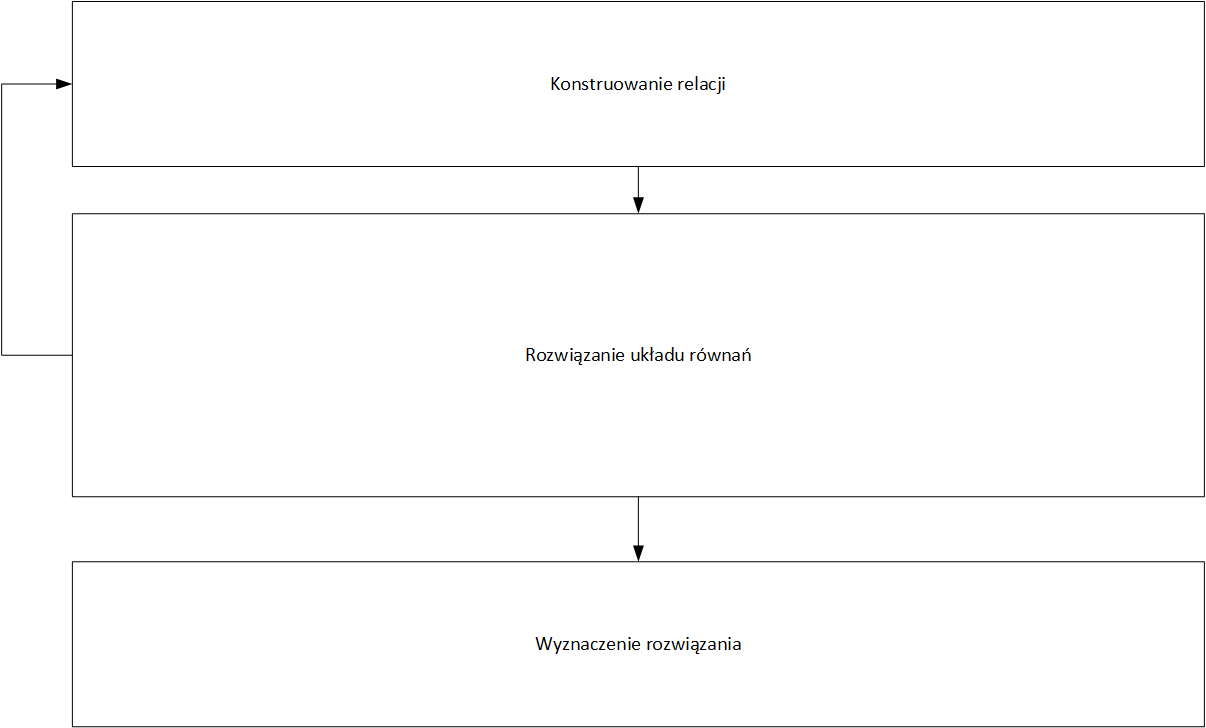
\includegraphics[width=10cm]{./img/schemat_1.png}
			\caption{Schemat blokowy algorytmu metody indeksu}
		\end{center}
	\end{figure}

	\begin{figure}[h]
	\begin{center}
		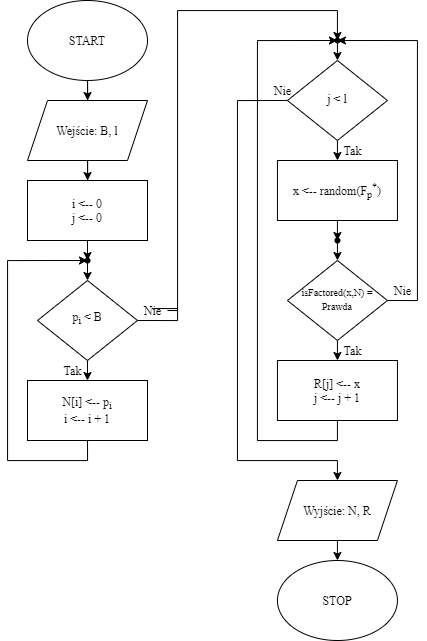
\includegraphics[width=10cm]{./img/2.png}
		\caption{Schemat blokowy algorytmu metody indeksu}
	\end{center}
\end{figure}

	\begin{figure}[h]
	\begin{center}
		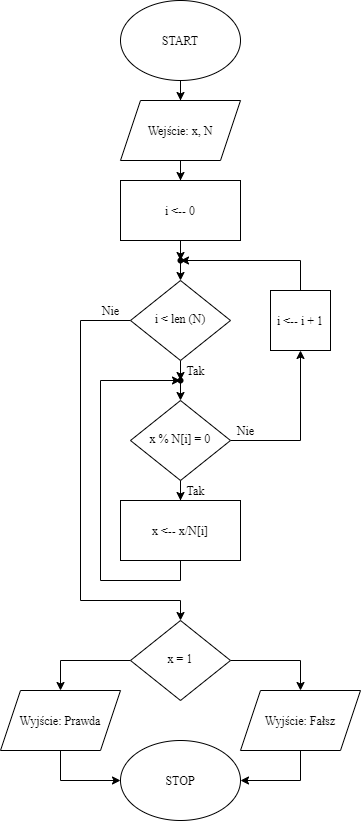
\includegraphics[width=9cm]{./img/3.png}
		\caption{Schemat blokowy algorytmu metody indeksu}
	\end{center}
\end{figure}


\end{document}
